\section{Applications}
\makesubcontentsslides

\subsection{RandSVD}
\makesubcontentsslidessec


\begin{frame}[fragile]
\fontsize{8pt}{10}\selectfont
\begin{block}{Randomized truncated SVD\footnotemark}
  \begin{minipage}{.56\textwidth}
    \begin{center}
      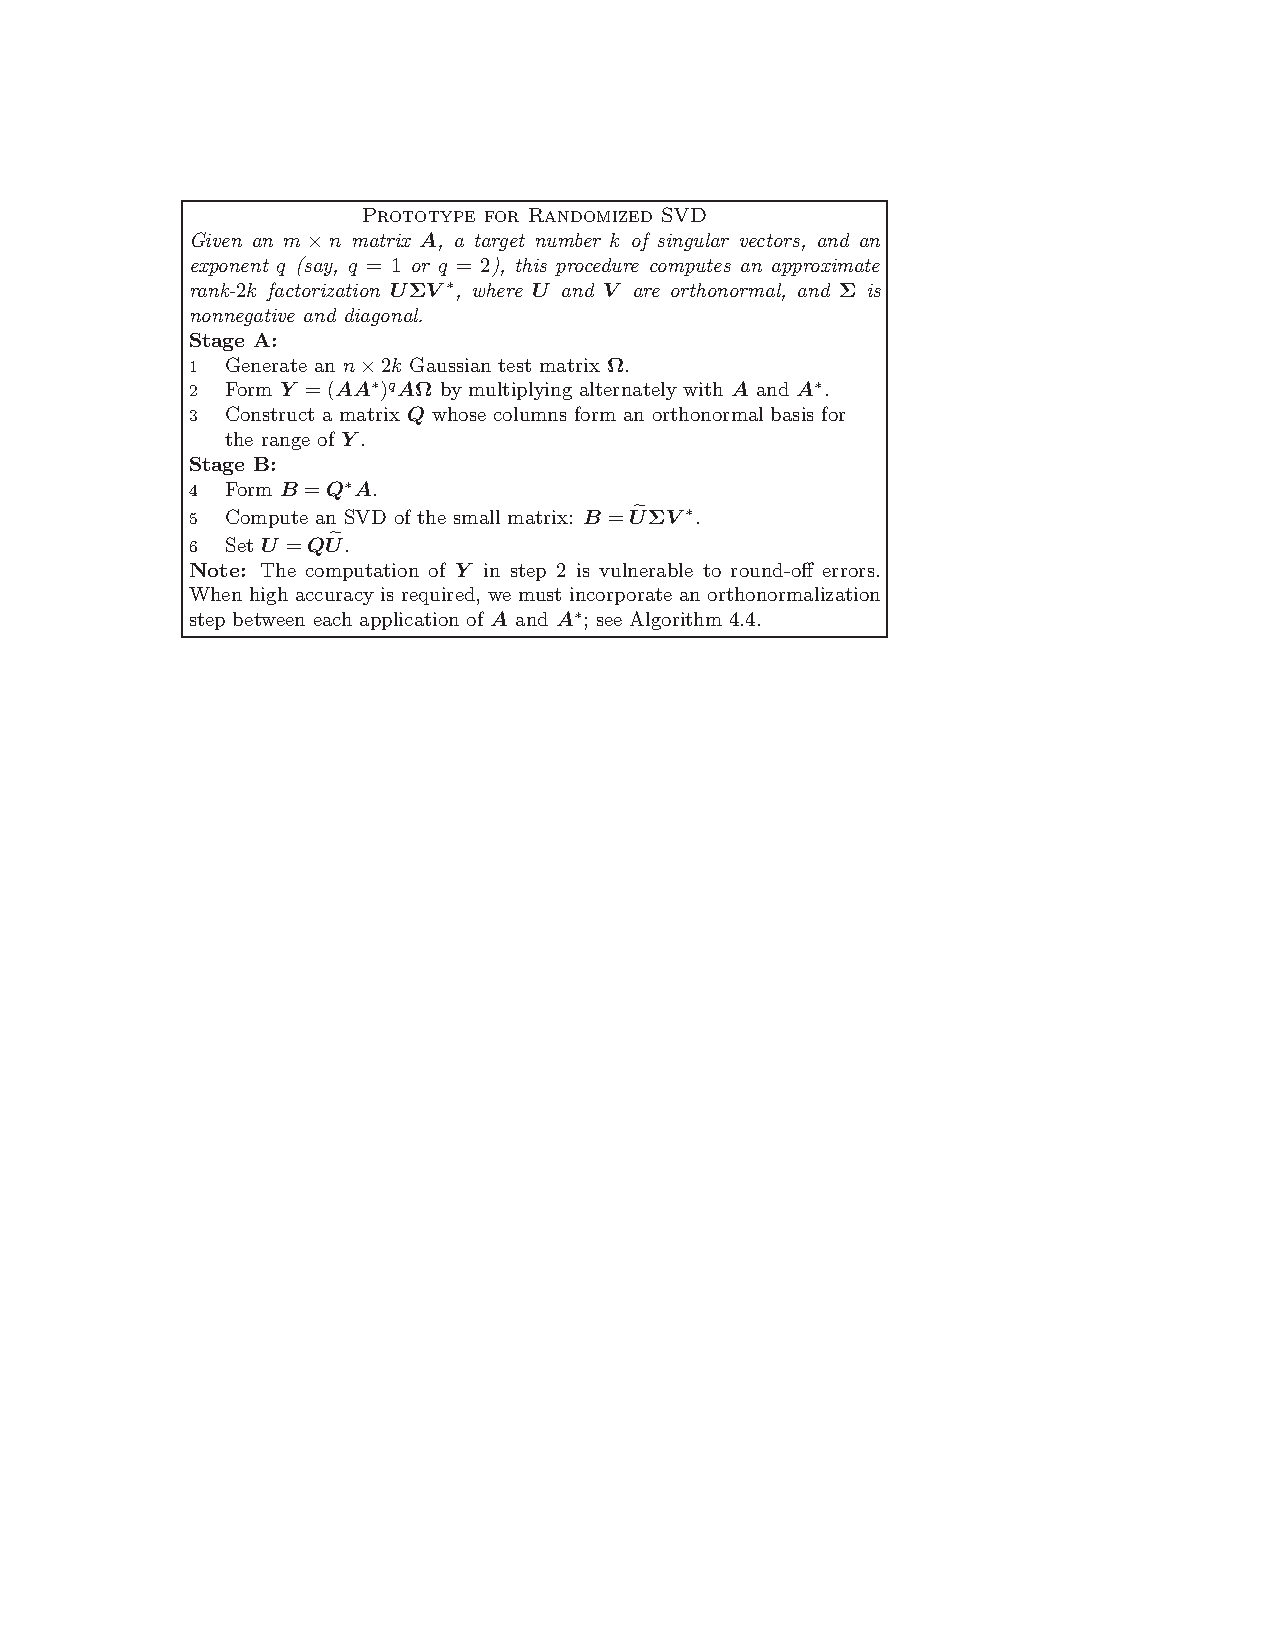
\includegraphics[height=.41\textheight]{../common/pics/randsvd/randSVDalg}
      \\
      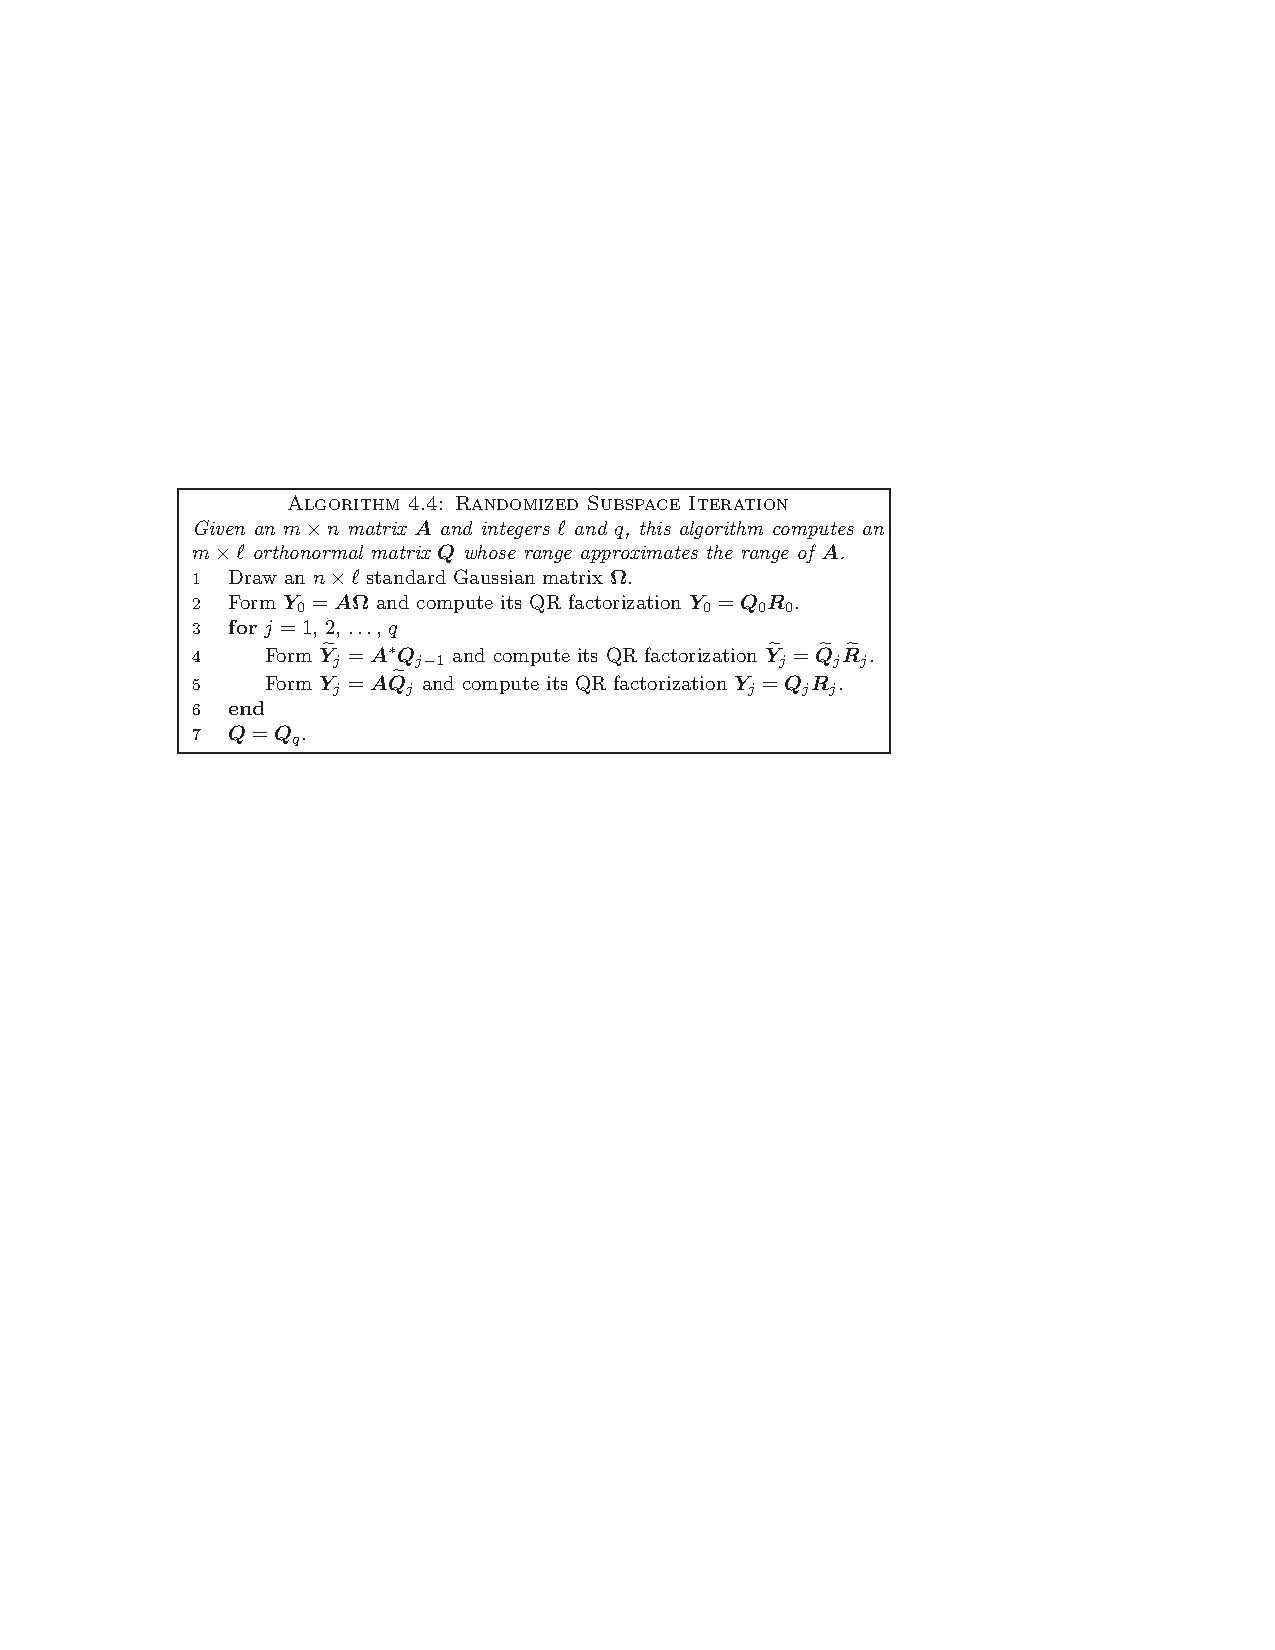
\includegraphics[height=.26\textheight]{../common/pics/randsvd/randSVDalg4_4}
    \end{center}
  \end{minipage}
%   \hspace{.01cm}
  \begin{minipage}{0.43\textwidth}
\begin{lstlisting}[title=Serial 
R,basicstyle=\tiny,backgroundcolor=\color{grayish} 
,numberstyle=\tiny\color{black},keywordstyle=\color{black},commentstyle=\color{ 
dkgreen},stringstyle=\color{black},escapeinside={(*@}{@*)}]
randSVD <- function(A, k, q=3)
  {
    ## Stage A
    Omega <- (*@ matrix(rnorm(n*2*k),@*)
      (*@ nrow=n, ncol=2*k) @*)
    Y <- A %*% Omega
    Q <- qr.Q(qr(Y))
    At <- t(A)
    for(i in 1:q)
      {
        Y <- At %*% Q
        Q <- qr.Q(qr(Y))
        Y <- A %*% Q
        Q <- qr.Q(qr(Y))
      }
    
    ## Stage B
    B <- t(Q) %*% A
    U <- La.svd(B)$u
    U <- Q %*% U
    U[, 1:k]
  }
\end{lstlisting} %balance$
\end{minipage}
{\fontsize{6pt}{10}\selectfont $^1$Halko, Martinsson, 
  and Tropp. 2011. Finding structure with randomness: probabilistic
  algorithms  for constructing \\[-1ex] approximate matrix decompositions
  \emph{SIAM Review} \textbf{53} 217--288}
\end{block}
\end{frame}


\begin{frame}[fragile]
 \fontsize{8pt}{10}\selectfont
\begin{block}{Randomized truncated SVD}
  \hfill
  \begin{minipage}{0.430\textwidth}
\begin{lstlisting}[title=Serial 
R,basicstyle=\tiny,backgroundcolor=\color{grayish} 
,numberstyle=\tiny\color{black},keywordstyle=\color{black},commentstyle=\color{ 
dkgreen},stringstyle=\color{black},escapeinside={(*@}{@*)}]
randSVD <- function(A, k, q=3)
  {
    ## Stage A
    Omega <- (*@ \textcolor{blue}{matrix(rnorm(n*2*k),} @*)
      (*@ \textcolor{blue}{ nrow=n, ncol=2*k)} @*)
    Y <- A %*% Omega
    Q <- qr.Q(qr(Y))
    At <- t(A)
    for(i in 1:q)
      {
        Y <- At %*% Q
        Q <- qr.Q(qr(Y))
        Y <- A %*% Q
        Q <- qr.Q(qr(Y))
      }
    
    ## Stage B
    B <- t(Q) %*% A
    U <- La.svd(B)$u
    U <- Q %*% U
    U[, 1:k]
  }
\end{lstlisting} %balance$
  \end{minipage}
  \hfill
  \begin{minipage}{0.430\textwidth}
\begin{lstlisting}[title=Parallel pbdR,basicstyle=\tiny,backgroundcolor=\color{
grayish}, numberstyle=\tiny\color{black},keywordstyle=\color{black},
commentstyle=\color{dkgreen},stringstyle=\color{black},escapeinside={(*@}{@*)}]
randSVD <- function(A, k, q=3)
  {
    ## Stage A
    Omega <- (*@ \textcolor{blue}{ddmatrix("rnorm",} @*)
      (*@ \textcolor{blue}{nrow=n, ncol=2*k)} @*)
    Y <- A %*% Omega
    Q <- qr.Q(qr(Y))
    At <- t(A)      
    for(i in 1:q)
      {
        Y <- At %*% Q   
        Q <- qr.Q(qr(Y))
        Y <- A %*% Q    
        Q <- qr.Q(qr(Y))
      }
    
    ## Stage B
    B <- t(Q) %*% A     
    U <- La.svd(B)$u 
    U <- Q %*% U     
    U[, 1:k]
  }
\end{lstlisting}  % balancing $
  \end{minipage}
\hfill
\end{block}
\end{frame}

\begin{frame}
  \begin{block}{From journal to scalable code and scaling data in one day.}
    \begin{center}
      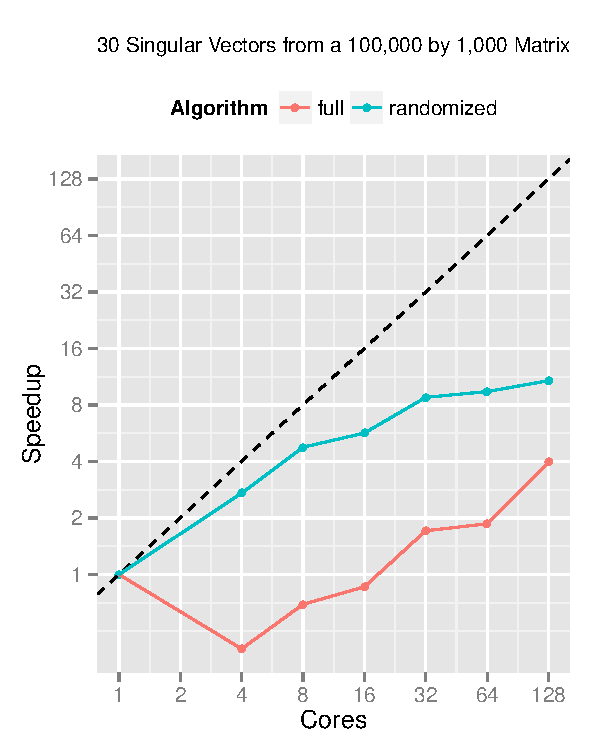
\includegraphics[width=.4\textwidth]{../common/pics/randsvd/randSVDspeedup}
      \hspace{1cm}
      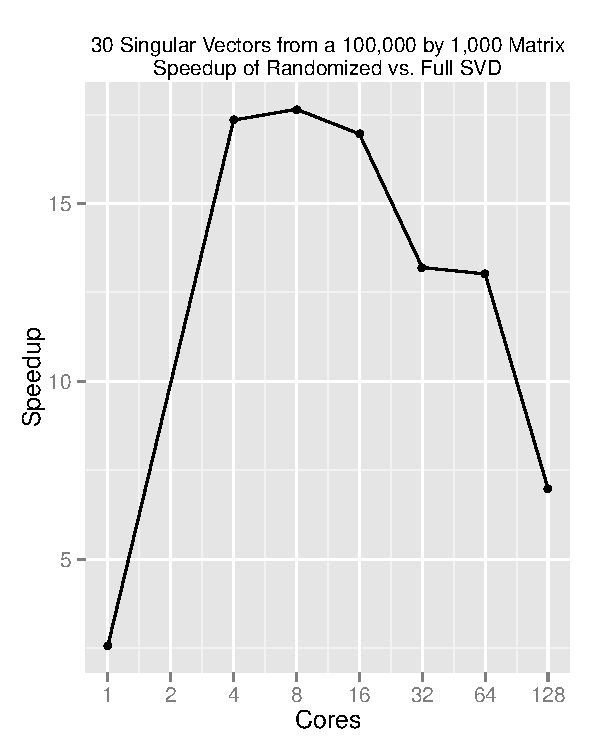
\includegraphics[width=.4\textwidth]{../common/pics/randsvd/randSpeedupSVD}
    \end{center}
  \end{block}
\end{frame}

\subsection{Precipitation Extremes in Climate Simulation Data}
\begin{frame}
  \begin{block}{\pkg{pmclust}: EM algorithm for Gaussian mixture
      model clustering}
    \begin{minipage}{6cm}\scriptsize
      \begin{itemize}
      \item High resolution (~25 km) atmospheric model, CAM 5.1
      \item Start with 2.9 TB, read and subset to extremes of 4 variables with
        256 cores
      \item Using multiple starts and Rand index, determine number of clusters
      \item Describes patterns of extreme precipitation across
        atmospheric layers of moisture, temperature, and wind velocity
      \end{itemize}
    \end{minipage}
    \begin{minipage}{5.8cm}
      \includegraphics[height=3.8cm]{pics/T_K_04_R_05}
      \includegraphics[height=3.8cm]{pics/Q_K_04_R_05}
      \includegraphics[height=3.8cm]{pics/OMEGA_K_04_R_05}
    \end{minipage}
    \vspace{-4.5ex}
    \begin{center}
      \includegraphics[trim=2mm 0mm 3mm 0mm,clip=true,height=3.4cm]{pics/tiles_4d_all_sort}
      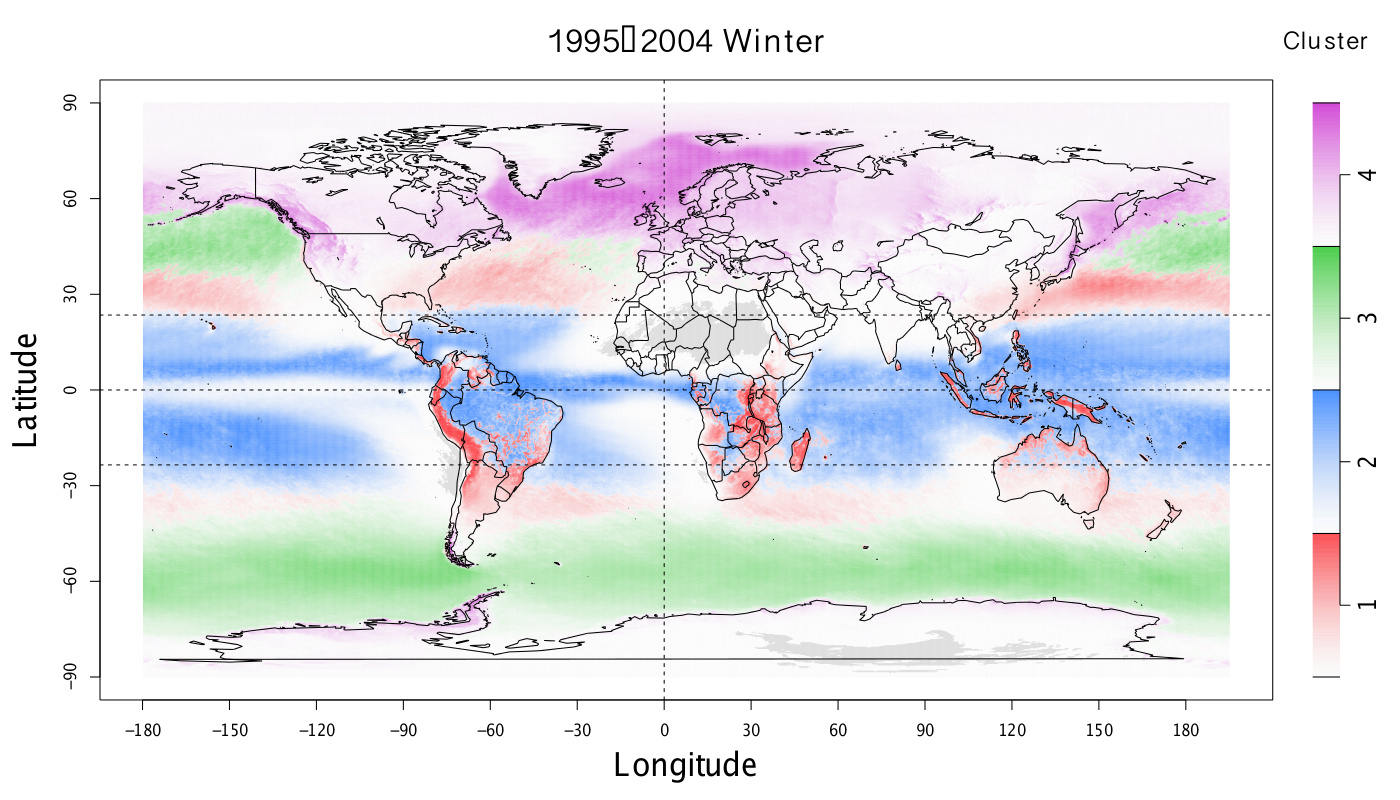
\includegraphics[height=3cm]{pics/map_K_04_R_05}
      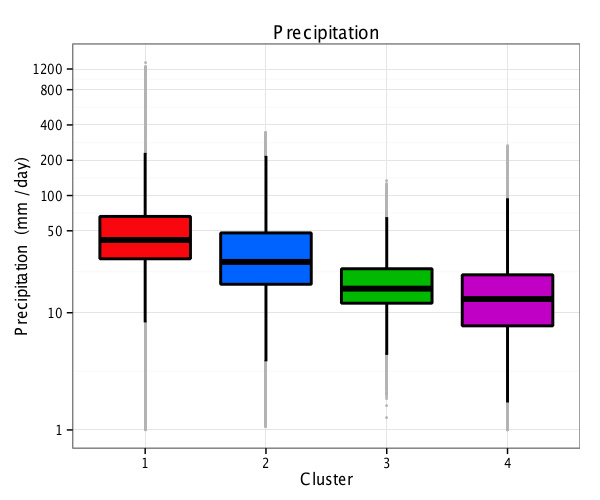
\includegraphics[trim=0mm 0mm 2mm 0mm,clip=true,height=3cm]{pics/PRECT_K_04_R_05}
    \end{center}
      \end{block}
\tiny Chen, Ostrouchov, Pugmire, Prabhat, and Wehner (2013). A
Parallel EM Algorithm for Model-Based Clustering \\[-2ex] Applied to the
Exploration of Large Spatio-Temporal Data. Technometrics {\bf 55}, p.513-523.
\end{frame}

\subsection{Ocean Turbulence Characterization}
\begin{frame}
  \begin{block}{Principal components analysis}
    \begin{itemize}\scriptsize
    \item Ocean turbulence data (2013 INCITE), 70GB per time step,
      interactive with 128 cores 
    \item Variability analysis quantifies organization into large
      coherent structures: for 99\% variability, 250 components needed at T=1
      but only 50 needed at T=30
    \end{itemize}
    \vspace{-3ex}
    \begin{center}
      \includegraphics[trim=.8cm 11.5cm 0.6cm 0cm,clip=true,height=3.8cm]{pics/TurbulencePCA}
    \end{center}
  \end{block}
  \begin{raggedright}\tiny
    Ostrouchov, Pugmire, Rosenberg, Chen, and Pouquet (2013)
    Computation and volume rendering of large-scale EOF \\[-2ex] coherent modes
    in rotating turbulent flow data, AGU Fall Meeting, December, 2013.
  \end{raggedright}
\end{frame}

\subsection{Biogeography models}

\begin{frame}
  \begin{block}{Biogeography matrix exponentiation}
    \begin{minipage}{5cm}
      \begin{itemize}\tiny
      \item Fitting biogeography models requires many matrix exponentiations
      \item Benchmark: Matrix exponential of 5000$\times$5000 matrix.
      \item R 3.1.0, Matrix 1.1-2, rexpokit 0.25, pbdDMAT 0.3-0
      \item Libs: Cray LibSci, NETLIB ScaLAPACK, Compilers: gnu 4.8.2
      \item Configuration: 1 thread == 1 MPI rank == 1 physical core
      \end{itemize}
      \vspace{-4ex}
      \begin{center}
        \includegraphics[trim=4cm 2cm 3.5cm 2.2cm,clip=true,height=4cm]{pics/Biogeography}
      \end{center}
    \end{minipage}
    \begin{minipage}{6.9cm}
      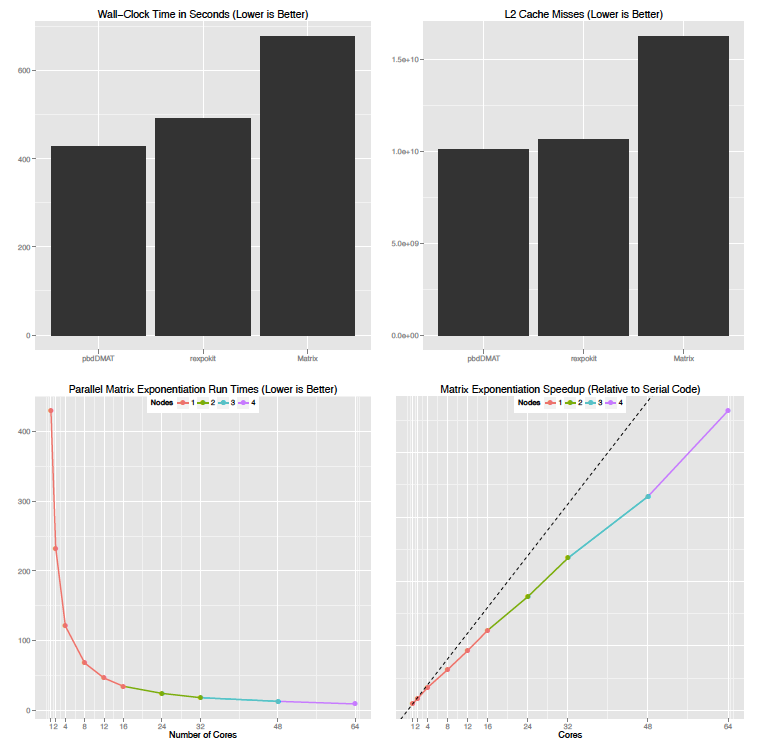
\includegraphics[trim=1mm 1mm 1mm 1mm,clip=true,height=7cm]{pics/MatExp}
    \end{minipage}
  \end{block}
  \begin{raggedright}\tiny
    Schmidt and Matzke (2014) Distributed matrix exponentiation, The R
    User Conference (UseR! 2014), \\[-2ex] Los Angeles, CA, August 2014 .
  \end{raggedright}
\end{frame}
